\begin{landscape}
\section{Evidencias nuevas del equipo}
\label{sec:evidencias-equipo}
Las imágenes siguientes se incorporan sin editar. Las capturas de
medición de Angel muestran la ruta del usuario; el equipo y la fecha
se documentan en su captura de entorno y metadatos. Se distinguen
de las capturas que contienen toda la identificación en una sola vista.
La captura de Steven en terminal se incluye en la sección de Lamport;
su imagen anterior en Bloc de notas se conserva en el repositorio
como apoyo documental y no se presenta como ejecución en terminal.

\begin{center}
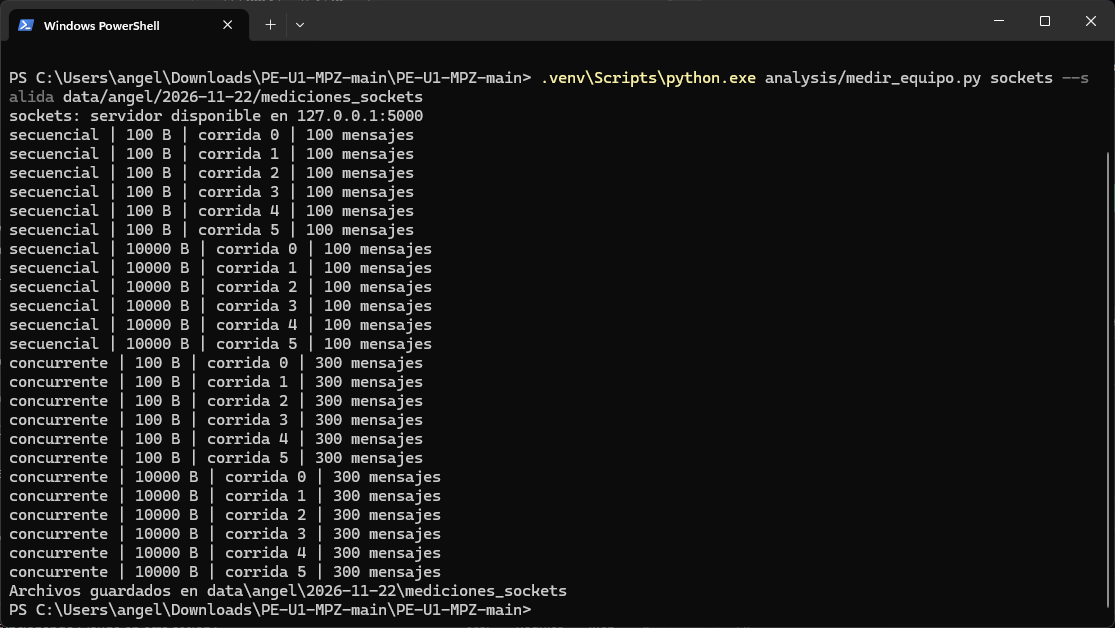
\includegraphics[width=\linewidth,height=0.74\textwidth,keepaspectratio]{../evidencias/01-latencias-sockets.png}
\captionof{figure}{Angel, 22/11: corridas de sockets con calentamiento y cinco repeticiones válidas por condición.}
\end{center}\end{landscape}
\begin{landscape}\begin{center}
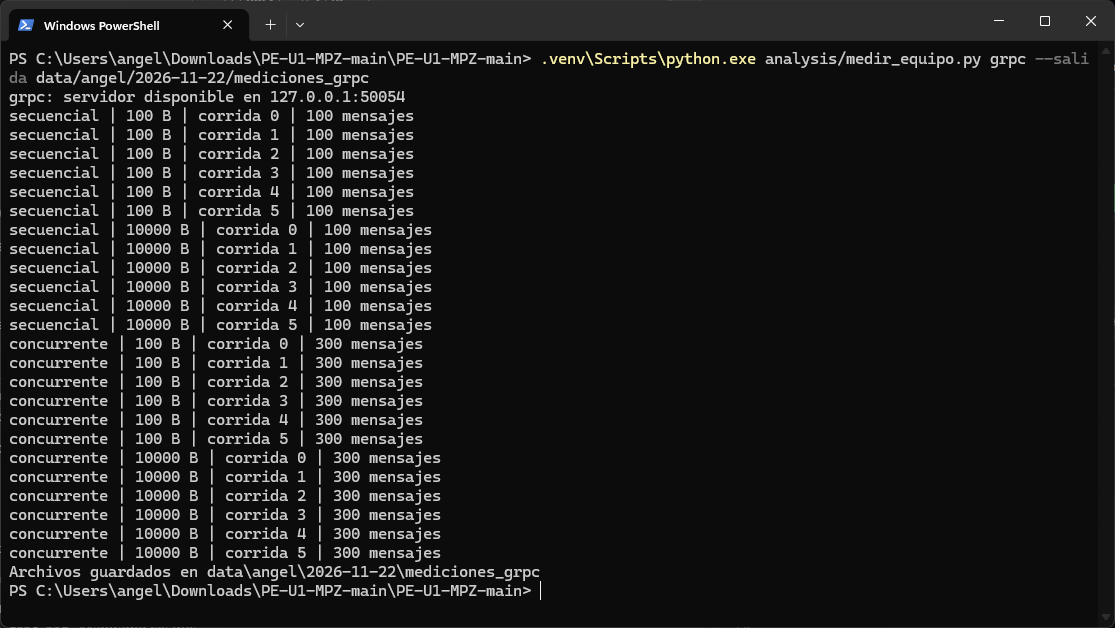
\includegraphics[width=\linewidth,height=0.85\textwidth,keepaspectratio]{../evidencias/02-latencia-grpc.png}
\captionof{figure}{Angel, 22/11: corridas secuenciales y concurrentes de gRPC.}
\end{center}\end{landscape}
\begin{landscape}\begin{center}
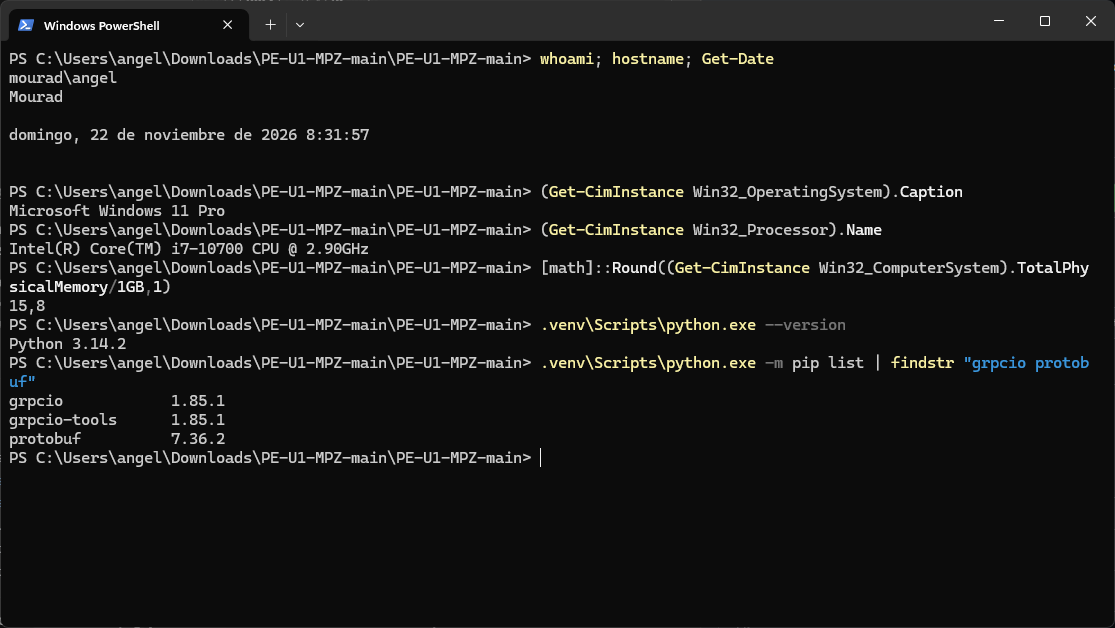
\includegraphics[width=\linewidth,height=0.85\textwidth,keepaspectratio]{../evidencias/03-entorno.png}
\captionof{figure}{Entorno de Mourad: usuario, equipo, fecha, sistema y versiones.}
\end{center}\end{landscape}
\begin{landscape}\begin{center}
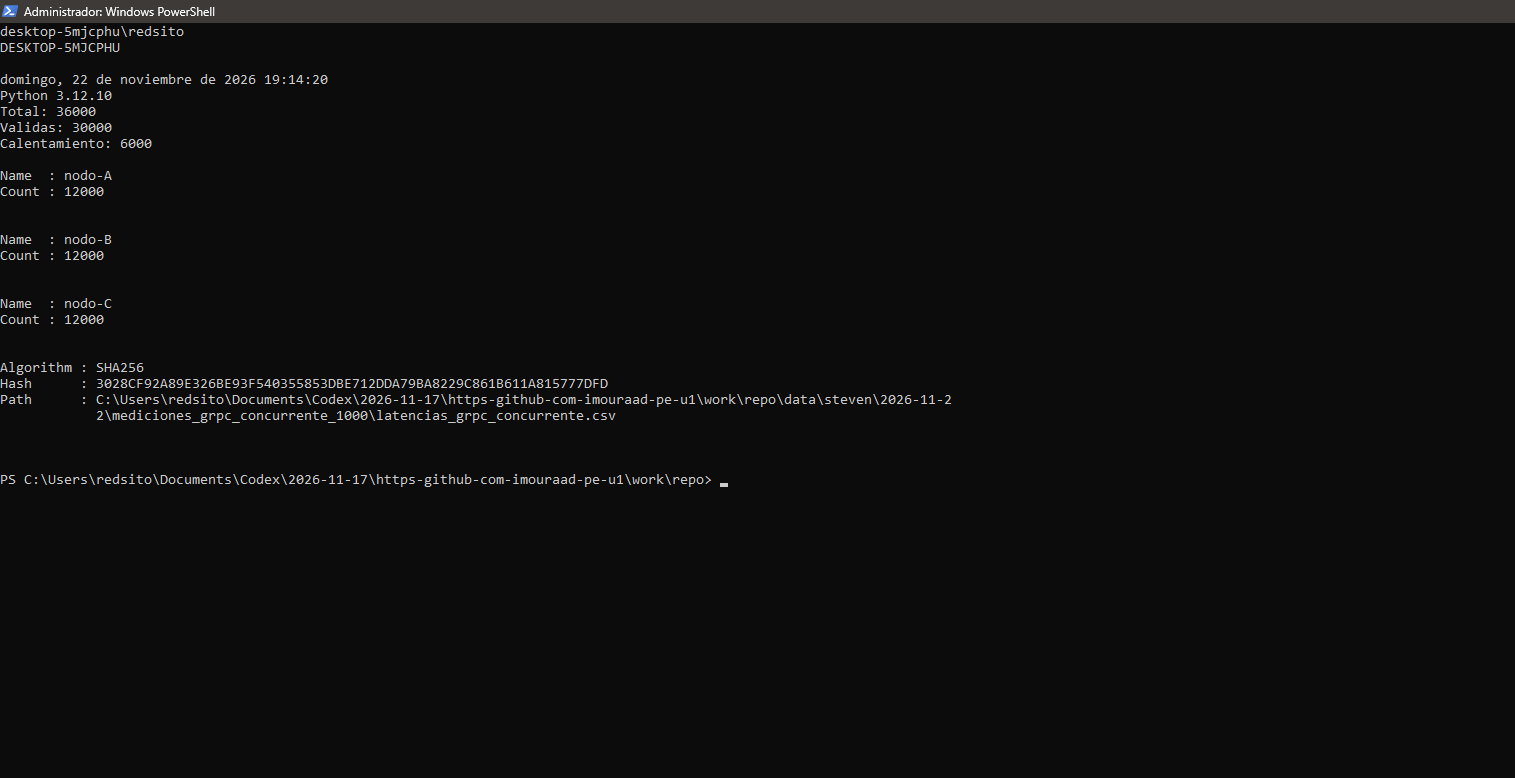
\includegraphics[width=\linewidth,height=0.85\textwidth,keepaspectratio]{../evidencias/steven/2026-11-22/grpc-concurrente-1000.png}
\captionof{figure}{Steven, 22/11: sesión gRPC concurrente con cinco corridas válidas por tamaño y 1\,000 envíos por cliente. Se muestran identificación, conteos y SHA-256.}
\end{center}\end{landscape}
